\paragraph{}
With the goal to detect facial expressions in images, we need to detect faces within them then extract their features so we have expectations on the input image to have good quality, sharpness, clearness as much as possible.\newline
Fortunately nowadays cameras have higher quality so quality, clearness or noise shouldn’t naturally cause a problem, however in case of low quality input photos we need to apply some enhancement techniques on them to achieve our goal.

\paragraph{}
\textbf{Most common problem and their enhancement techniques:}\newline

\paragraph{}
\textbf{Salt and Pepper Noise:}\newline
It is a form of noise sometimes seen on images. It is also known as impulse noise. This noise can be caused by sharp and sudden disturbances in the image signal. It presents itself as sparsely occurring white and black pixels.\newline
An effective noise reduction method for this type of noise is a Median Filter.\newline
The main idea of the Median Filter is to run through the photo entry(Pixel) by entry, replacing each entry with the median of neighboring entries. The pattern of neighbors is called the "window", which slides, entry by entry, over the entire photo.

\begin{figure}[H]
	\centering
	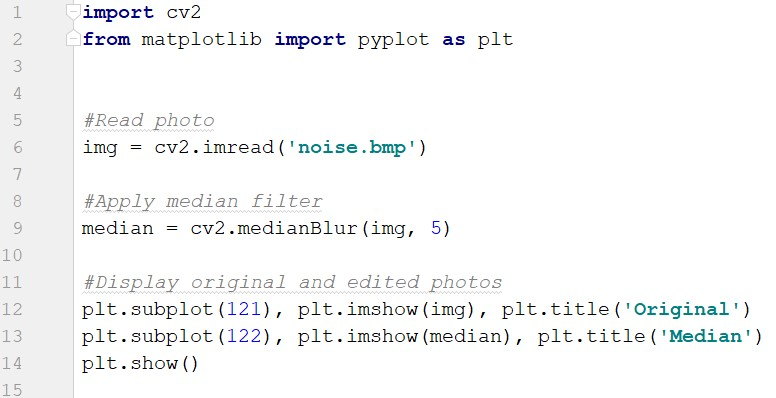
\includegraphics[width=\linewidth]{median_code.jpg}
	\caption{Median Code Example}
\end{figure}

\begin{figure}[H]
	\centering
	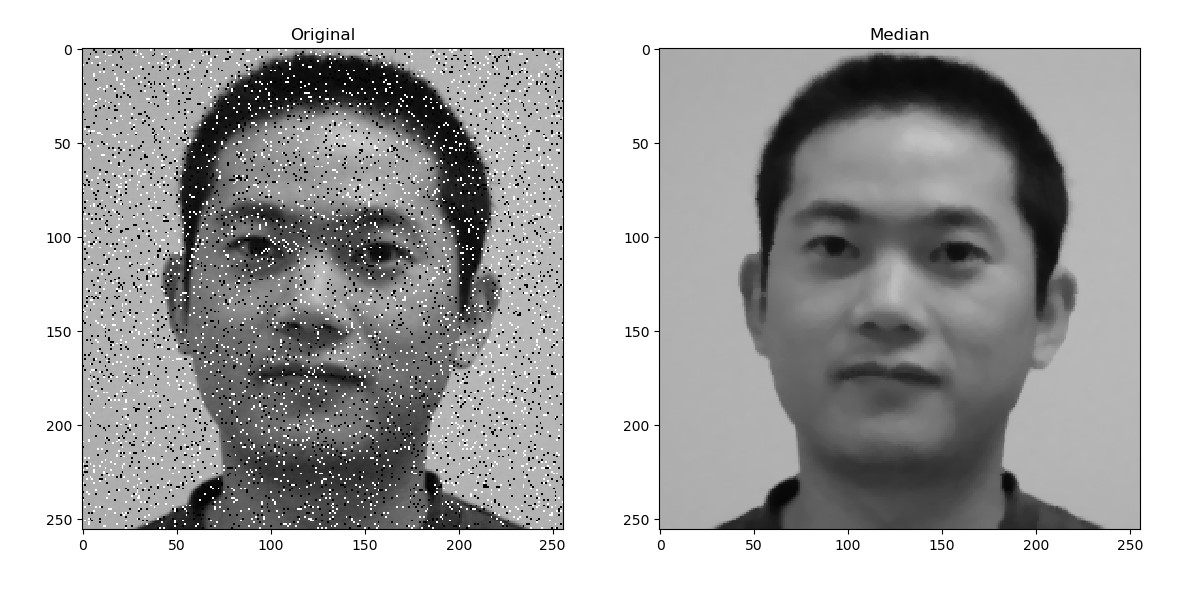
\includegraphics[width=\linewidth]{salt_pepper.jpg}
	\caption{I/O Example}
\end{figure}

\paragraph{}
\textbf{Gaussian Noise:}\newline
It is a statistical noise having a probability density function (PDF) equal to that of the normal distribution, which is also known as the Gaussian distribution. In other words, the values that the noise can take on are Gaussian-distributed.\newline
An effective noise reduction method for this type of noise is a Non-local Means Denoising Algorithm.\newline
It works as we need a set of similar images to average out the noise. Consider a small window (say 5x5 window) in the image. Chance is large that the same patch may be somewhere else in the image. Sometimes in a small neighborhood around it. What about using these similar patches together and find their average.\newline
See an example image below:\newline
\begin{figure}[H]
	\centering
	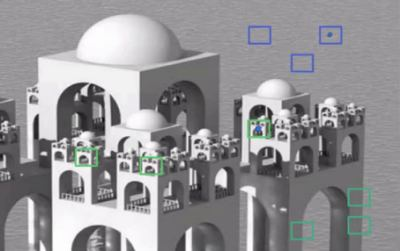
\includegraphics[width=\linewidth]{nlmd.jpg}
\end{figure}
The blue patches in the image looks the similar. Green patches looks similar. So we take a pixel, take small window around it, search for similar windows in the image, average all the windows and replace the pixel with the result we got.\newline
But we did not use it as it is slow and this will make problem in real-time streaming.

\begin{figure}[H]
	\centering
	\includegraphics[width=\linewidth]{denoising_code.jpg}
	\caption{Denoising Code Example}
\end{figure}

\begin{figure}[H]
	\centering
	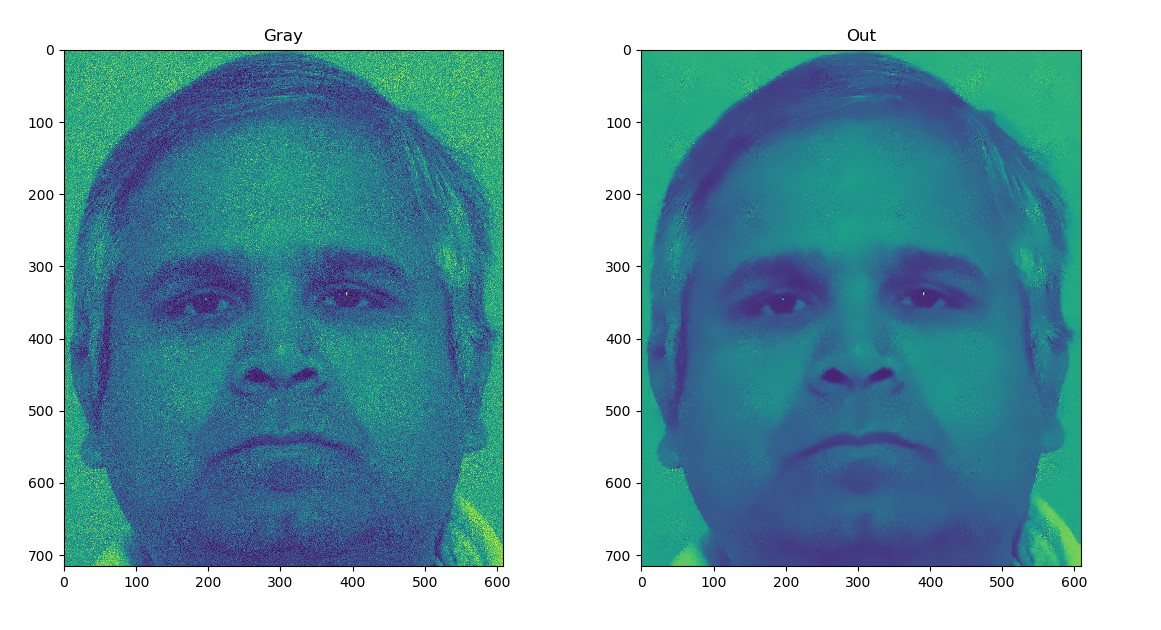
\includegraphics[width=\linewidth]{gaussian.jpg}
	\caption{I/O Example}
\end{figure}

\paragraph{}
\textbf{Smoothed Images:}\newline
It is images which have a smoothed(blurred) effect on them which blur small details.\newline
An effective noise reduction method for this type of noise is a Laplacian Filter (Sharpening Spatial Filter).\newline
Sharpening spatial filters seek to highlight small details by:\newline
– Remove blurring from images\newline
– Highlight edges\newline
Sharpening filters are based on spatial differentiation.\newline
The Laplacian is defined as follows:\newline
\[\nabla^{2} f = \frac{\partial^{2}f}{\partial^{2}x} + \frac{\partial^{2}f}{\partial^{2}y}\]

\paragraph{}
where the partial 2nd order derivative in the x direction is defined as follows:\newline
\[\frac{\partial^{2}f}{\partial^{2}x} = f(x+1, y) + f(x-1, y) - 2f(x, y)\]

\paragraph{}
and in the y direction as follows:\newline
\[\frac{\partial^{2}f}{\partial^{2}x} = f(x, y+1) + f(x, y-1) - 2f(x, y)\]

\paragraph{}
So, the Laplacian can be given as follows:\newline
\[\nabla^{2} f = f(x+1, y) + f(x-1, y) + f(x, y+1) + f(x, y-1) - 4f(x, y)\]

\paragraph{}
We can transform that to:\newline
\begin{figure}[H]
	\centering
	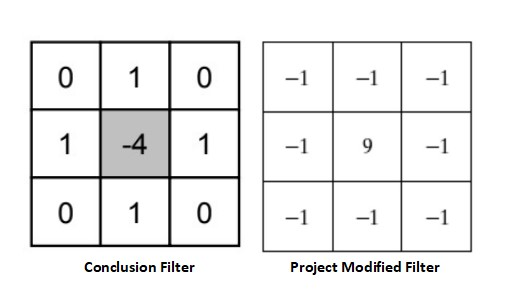
\includegraphics[width=\linewidth]{filters.jpg}
\end{figure}

The main idea of the Laplacian Filter is to run through the photo entry(Pixel) by entry, replacing each entry with the sum of multiplaied entries of original window of image by the filter(kernel).
\begin{figure}[H]
	\centering
	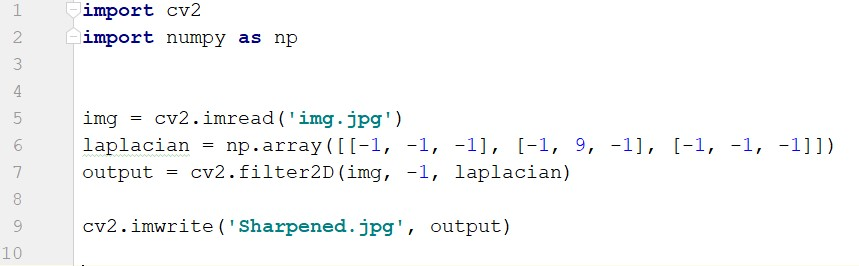
\includegraphics[width=\linewidth]{sharpening_code.jpg}
	\caption{Sharpening Code Example}
\end{figure}
\begin{figure}[H]
	\centering
	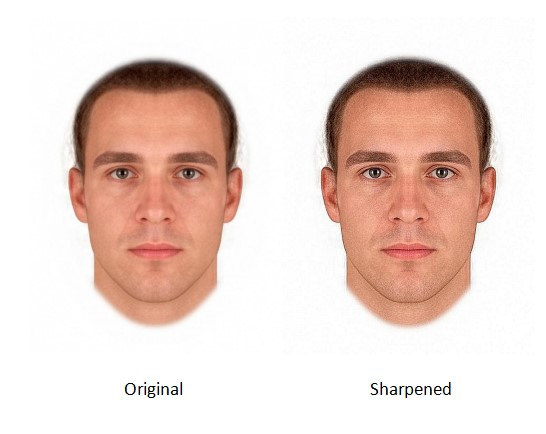
\includegraphics[width=\linewidth]{Sharpened.jpg}
	\caption{I/O Example}
\end{figure}

\paragraph{}
\textbf{Motion Blurred Images:}\newline
It is the apparent streaking of moving objects in an image or a sequence of frames, such as a film or animation. It results when the image being recorded changes during the recording of a single exposure, due to rapid movement or long exposure.\newline
An effective noise reduction method for this type of noise is a trained library called Keras Deblur GAN.\newline
But we did not use it as it is slow and this will make problem in real-time streaming.
\begin{figure}[H]
	\centering
	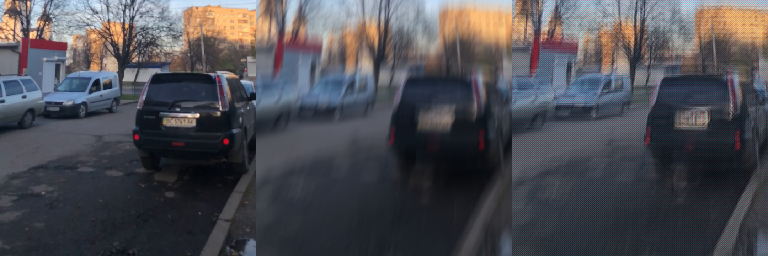
\includegraphics[width=\linewidth]{motion_blur.png}
	\caption{Motion Blur Example}
\end{figure}
\paragraph{}
\textbf{Rotated and Different Size Faces:}\newline
In out project we prefer to deal with aligned and scaled faces to easily detect them.\newline
We deal with this problem by using a trained model called FaceAligner in OpenCV library.\newline
It works as photo rotated that such the eyes lie on a horizontal line (i.e., the face is rotated such that the eyes lie along the same y-coordinates) and scaled such that the size of the faces are approximately identical.\newline
But we did not use it as it is slow and this will make problem in real-time streaming so we depend on frontal faces only.
\begin{figure}[H]
	\centering
	\includegraphics[width=\linewidth]{aligning.jpg}
	\caption{Aligning Example}
\end{figure}
\newpage
